\documentclass[12pt, letterpaper]{article}
\usepackage{graphicx} % Required for inserting images
\usepackage{hyperref}
\usepackage{listings}
\usepackage{amssymb}
\usepackage{amsmath}
\usepackage[english]{babel}
\usepackage{nicefrac, xfrac}
\usepackage{mathtools}
\newcommand{\acc}{\\\hphantom{}\\}
\usepackage[table,xcdraw]{xcolor}
\usepackage[paper=a4paper,left=20mm,right=20mm,bottom=25mm,top=25mm]{geometry}
\renewcommand{\labelenumii}{\arabic{enumi}.\arabic{enumii}}
    \renewcommand{\labelenumiii}{\arabic{enumi}.\arabic{enumii}.\arabic{enumiii}}
    \renewcommand{\labelenumiv}{\arabic{enumi}.\arabic{enumii}.\arabic{enumiii}.\arabic{enumiv}}
\title{Accademia 2 (gruppo 16)}
% \author{ Giacomo Biribicchi \and Marco Casu \and Christian Di Manno \and Alessandro Gautieri }
\date{}


\begin{document}

\maketitle


\section{Requisiti}

I dati di interesse per il sistema sono \underline{Docenti}, \underline{Progetti} ed \underline{Attività}.
\begin{enumerate}
    \item \textbf{Docente}\begin{enumerate}
        \item Nome 
        \item Cognome 
        \item Data di nascita 
        \item Matricola 
        \item Posizione universitaria
        \item Progetti alla quale partecipa
    \end{enumerate}
    \item \textbf{Progetto}\begin{enumerate}
        \item Nome 
        \item Acronimo 
        \item Codice progetto
        \item Data inizio 
        \item Data fine 
        \item Docenti coinvolti
        \item Work Package\begin{enumerate}
            \item Nome 
            \item Data inizio 
            \item Data fine
        \end{enumerate}
    \end{enumerate}
    \item\textbf{Attività}\begin{enumerate}
        \item Data 
        \item Durata in ore 
        \item tipologia impegno 
        \item motivazione
    \end{enumerate}
\end{enumerate}\newpage
\section{Considerazioni}
Ci sarà una classe \underline{TipologiaAttività}, un \underline{Attività} può essere di 
più tipologie.\acc Un \underline{Attività} può coinvolgere più \underline{Docenti}.\acc 
Il \underline{Docente}, tramite la relazione \textit{doc\_part}, segnala che in uno specifico 
intervallo temporale fa parte di un gruppo di realizzazione di un progetto, non indica però, i giorni 
specifici in cui un docente sarà assente per via di tale progetto, ciò, sarà dato dalla 
relazione dedicata nell'\underline{Attività} di tipo \underline{Progettuale}.\acc 
%Le assenza di un \underline{Docente} relative ad un \underline{Attività} di tipo  \underline{Progettuale},
%possono anche riferirsi ad un \underline{Progetto} alla quale il \underline{Docente} non partecipa.\acc 
%Nello specifico, un \underline{Docente} ha dei progetti nella quale è
Un \underline{Docente} può prendere parte ad un \underline{Attività} di tipo \underline{Progettuale} 
eslcusivamente riguardo un  \underline{Progetto} alla quale il \underline{Docente} partecipa.
\newpage
\section{UML}\begin{center}
    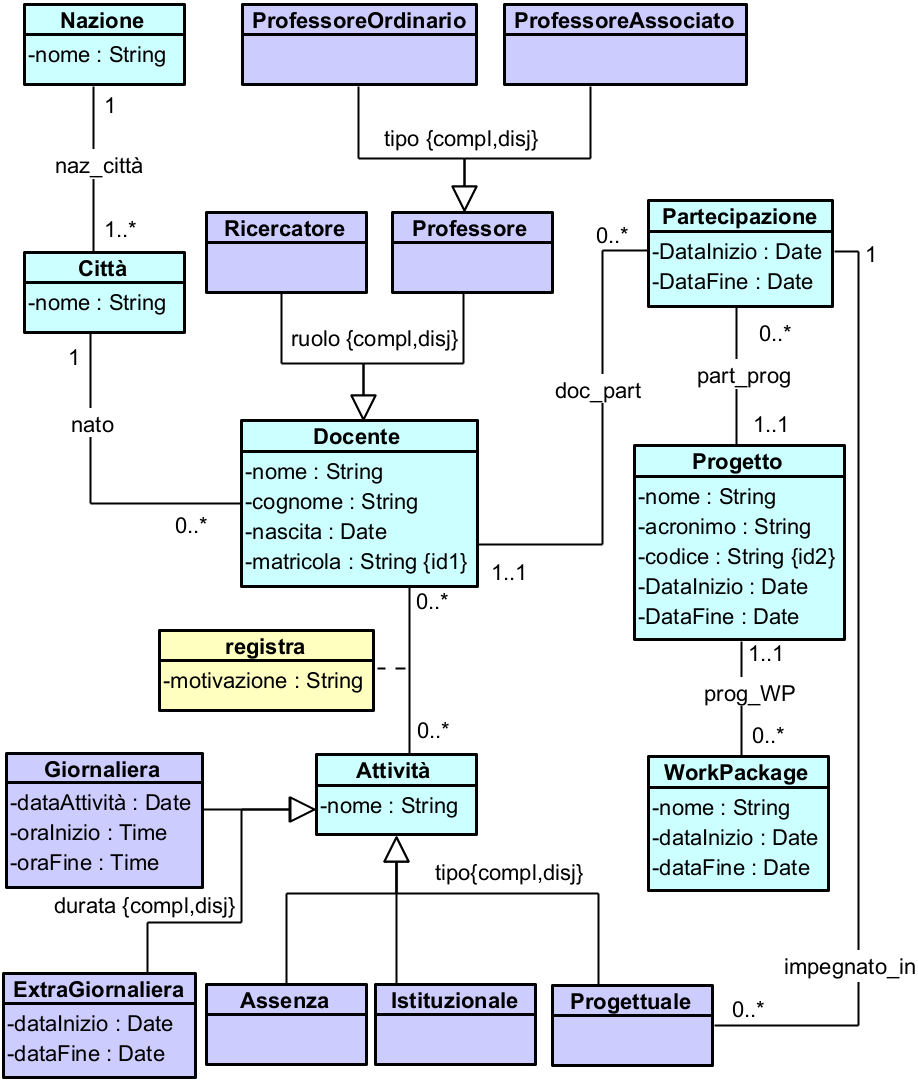
\includegraphics[width=1.1\textwidth]{images/UML.png}
\end{center}


\end{document}

